
% ====================================
% chapter 2
% ====================================
\chapter{BinaryConnectによる良否判定}

% ******************************************************
% NeuralNetwork
% ******************************************************
\section{Neural Network}
Neural Networkとはニューロンと呼ばれる人間の脳細胞をもとに作られた数理モデルである.入力に対し重みをかけた時の出力から入力の特徴を抽出し分類問題を解く機械学習の1種である.


\subsection{Neural Networkの構造}
Neural Networkはユニットと呼ばれる最小要素を持ち,それに対し複数の入力と重み,バイアスから計算結果を出力する.
これらは図\ref{fig_NN1}のような構造をしている.
\begin{align*}
y &= w_{1}x_{1} + w_{2}x_{2} + w_{3}x_{3} + b
\end{align*}
\begin{figure}[]
  \begin{center}
    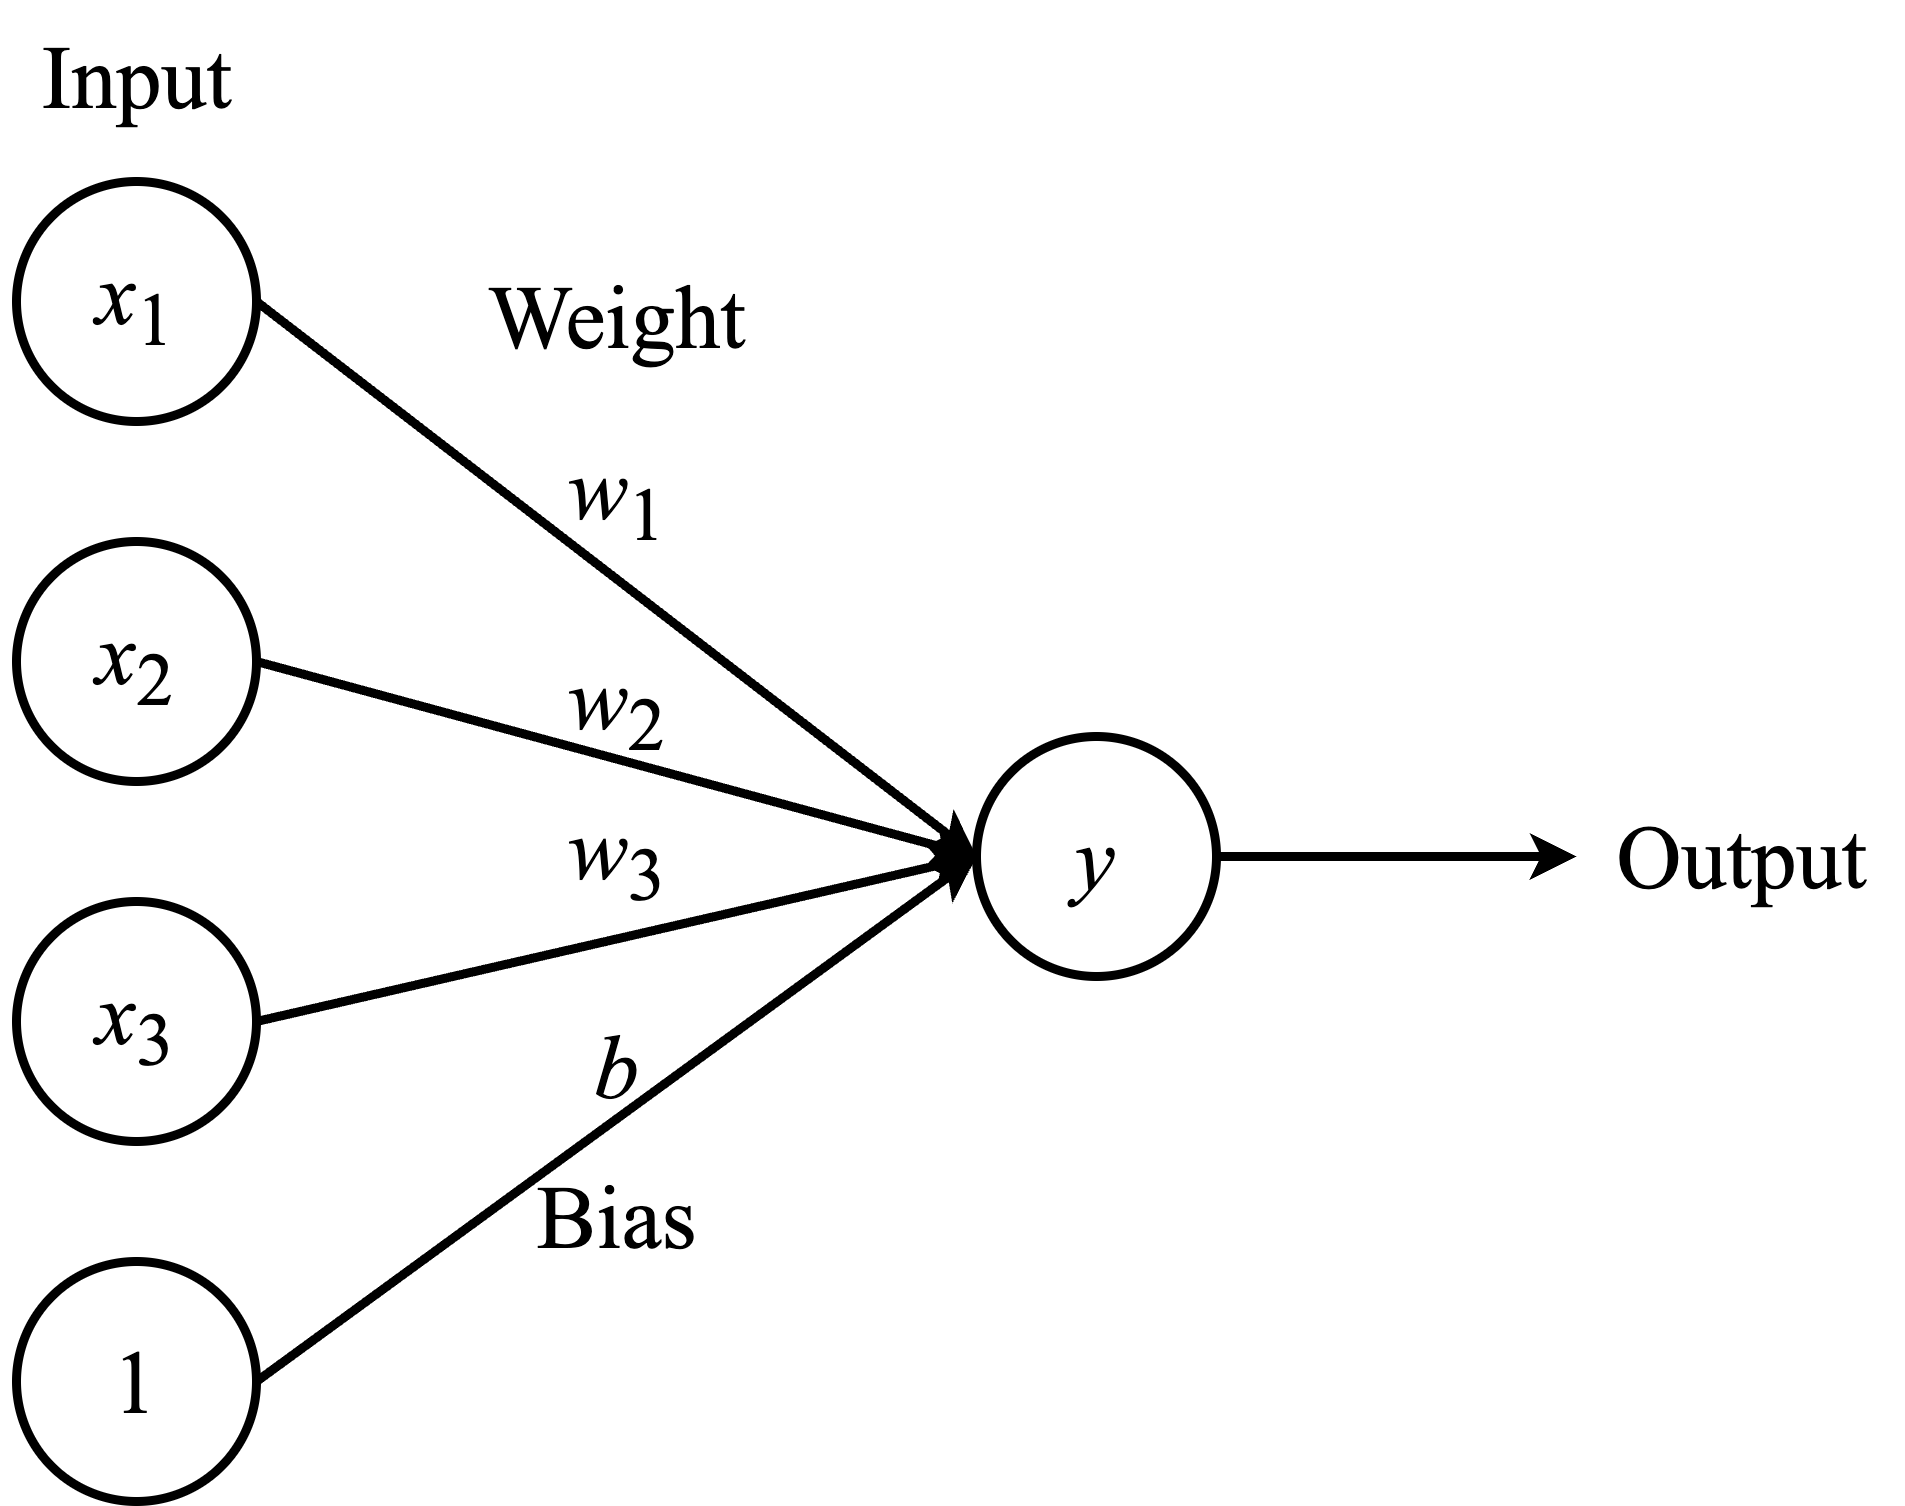
\includegraphics[scale = 0.1]{./chapter2/nn_1.png}
    \caption{ユニットの構造}
    \label{fig_NN1}
  \end{center}
\end{figure}
入力$x_i$に対し重み$w$を乗算したものにバイアス$b$を足すことで出力$y$を得る.計算式は以下のように表される.

ここで出力$y$を複数個にすると,図\ref{fig_NN}のような構造になる.ユニットの縦方向の集まりのことを層と呼び,Neural Networkはこの層を複数組み合わせ,入力層・中間層・出力層という層を形成し計算を行う.
入力層$x$のユニットの個数を$i=1,2,3\ldots I$,中間層$z$のユニットの個数を$j=1,2,3\ldots J$とすると,それぞれの重みは$w_{ji}$,バイアスは$b_j$となるため一般化した計算式は以下のようになる.
\begin{figure}[]
  \begin{center}
    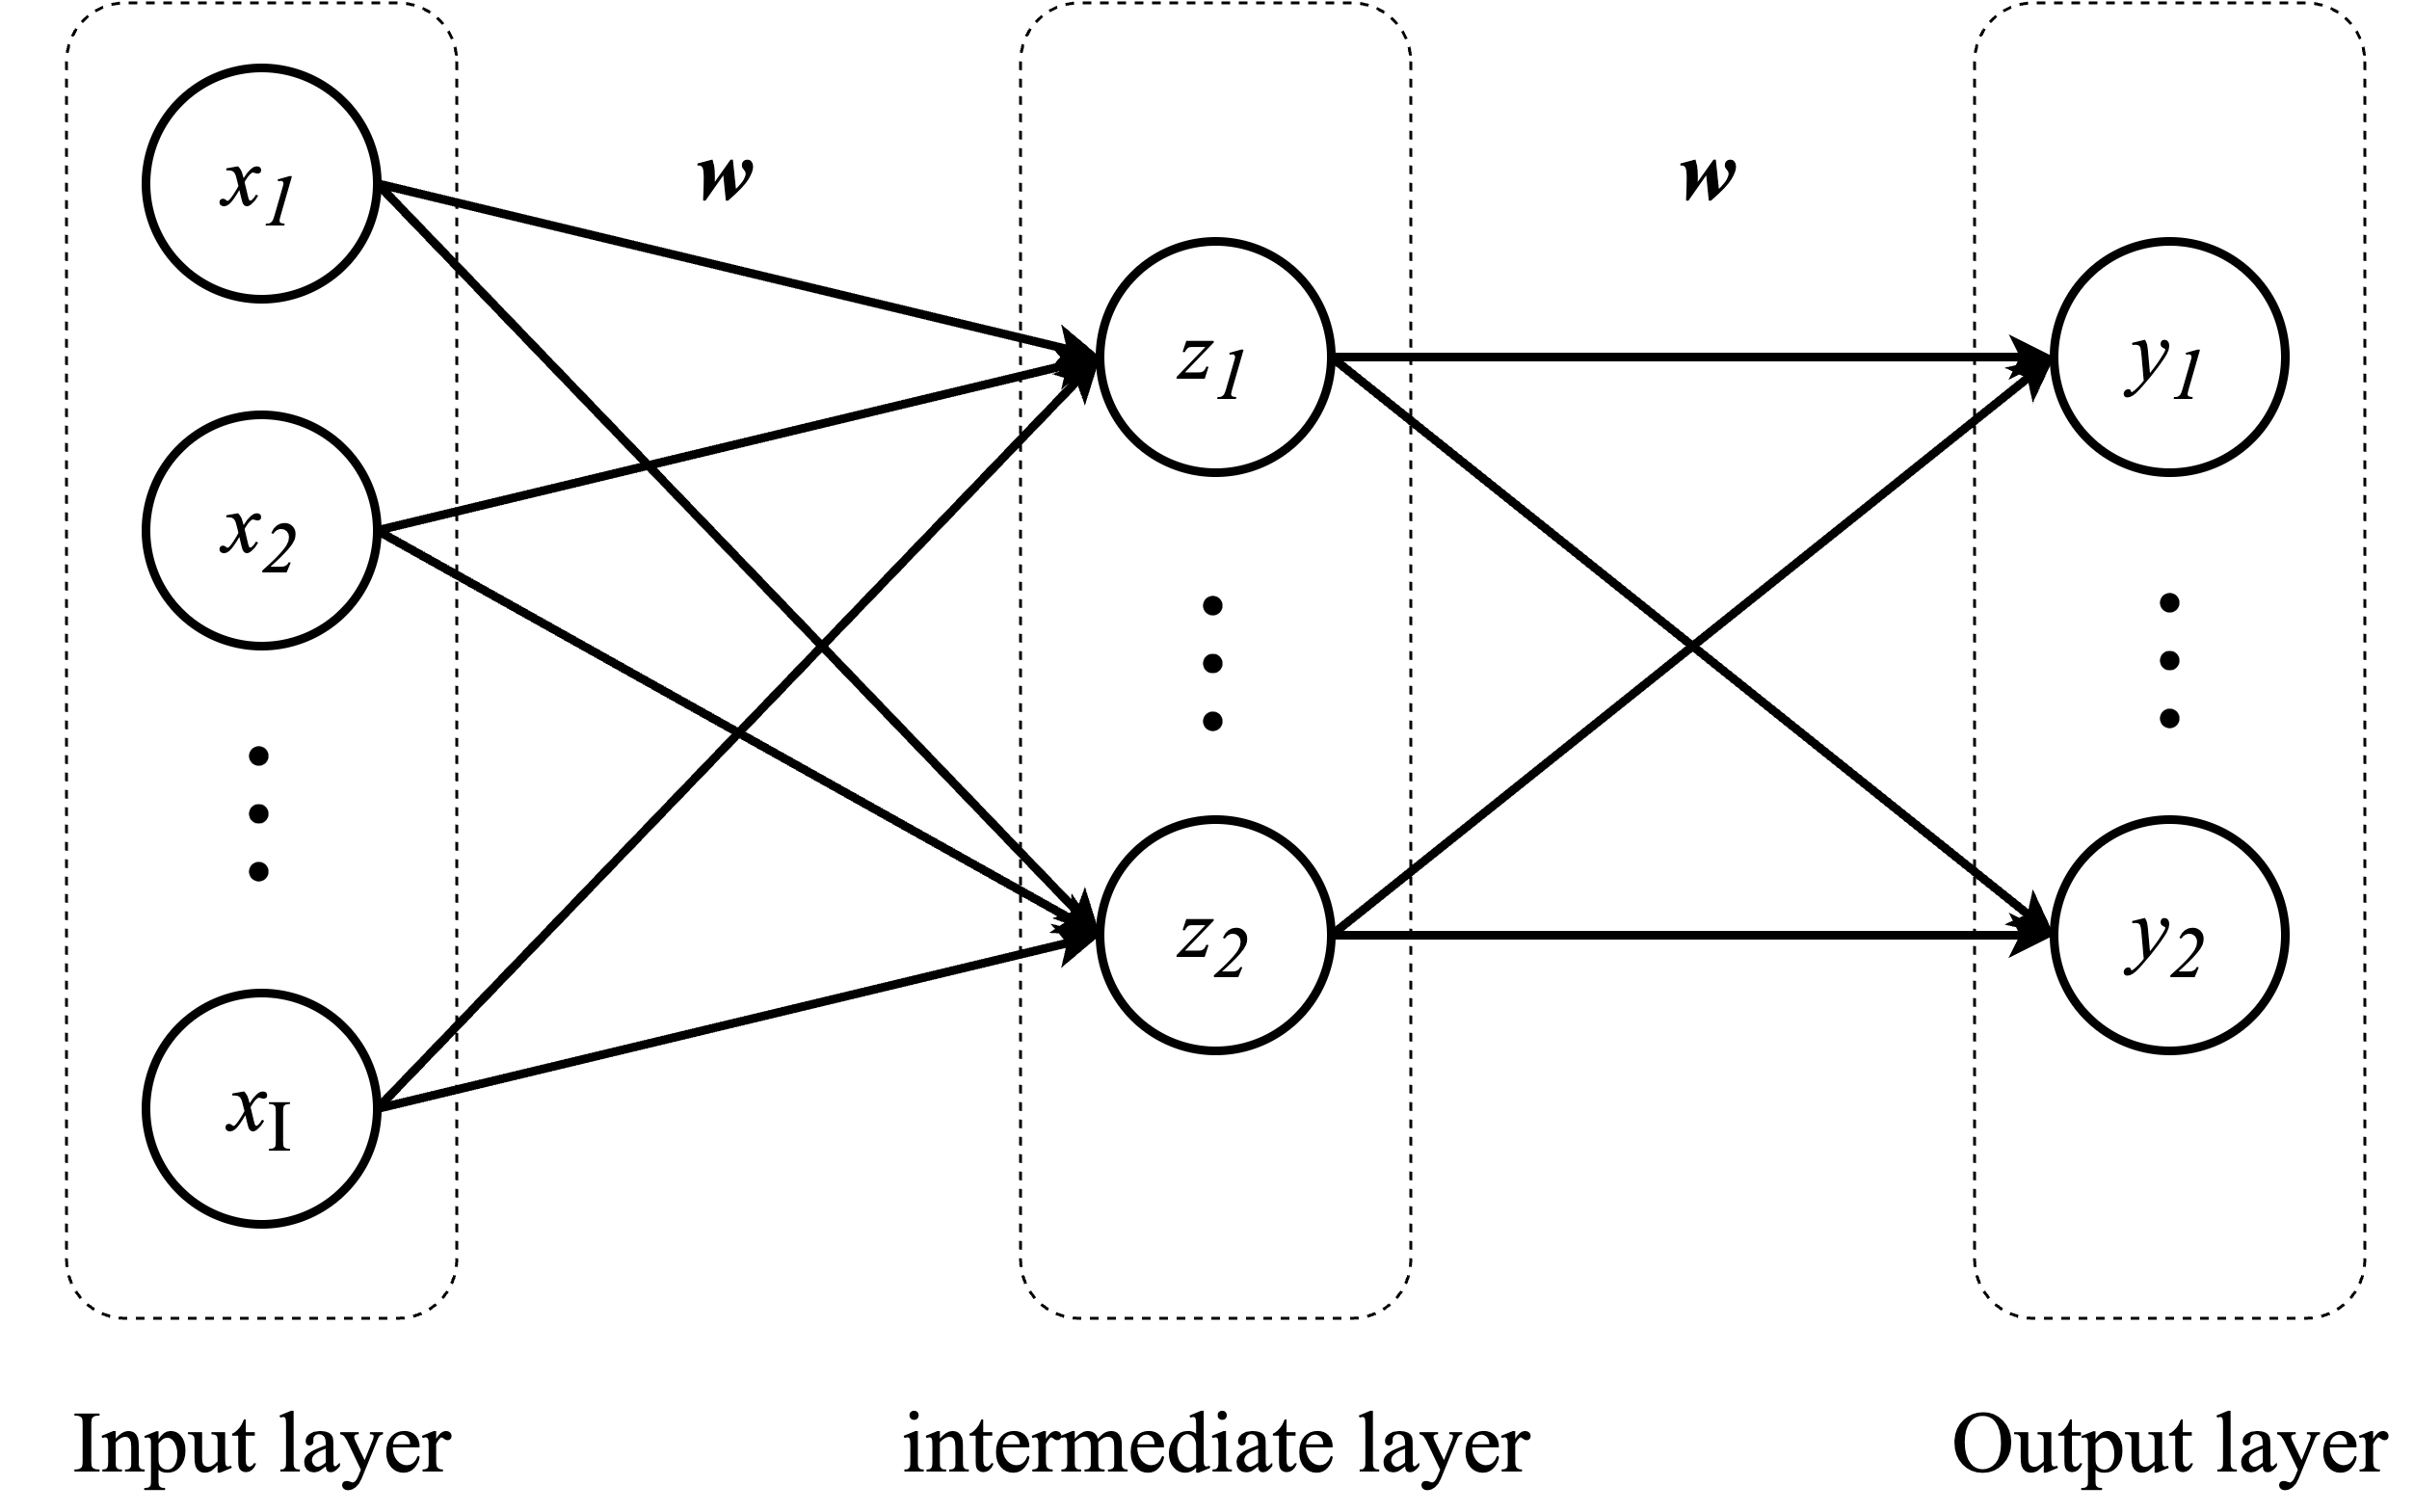
\includegraphics[scale = 0.1]{./chapter2/neural_network.png}
    \caption{Neural Networkの構造}
    \label{fig_NN}
  \end{center}
\end{figure}

\begin{align*}
z_{1} &= w_{11}x_{1} + w_{12}x_{2} + w_{13}x_{3} + b_1\\
z_{2} &= w_{21}x_{1} + w_{22}x_{2} + w_{23}x_{3} + b_2\\
z_{3} &= w_{31}x_{1} + w_{32}x_{2} + w_{33}x_{3} + b_3
\end{align*}

構造は学習モデルによって異なるため,必ずこのような形になるわけではない.そこで,入力の個数をI個とし,各要素をベクトルと行列を用いて表し,次の層のユニットへの出力を一般化すると以下のような式となる.
\begin{align*}
\bm{z} = \bm{W}\bm{x} + \bm{b}
\end{align*}

中間層は1層のみである必要はなく,中間層の出力を次の層への入力として扱うことで層を多数化し,入力層から出力層までに多数の隠れ層を追加する.層数$L$のネットワークが存在する時,$l+1$層のユニットの出力$\bm{z}^{(l+1)}$は$l$層のユニットの出力$\bm{z}^{(l)}$から計算されるため,
\begin{align*}
\bm{z}^{(l+1)} = \bm{W}^{(l+1)}\bm{z}^{(l)} + \bm{b}^{(l+1)}
\end{align*}
という式で一般化される.したがって$l=1,2,3\ldots L-1$までの計算を順に行なっていくことで各層の出力を得ることができ,最終的な出力$\bm{y}=\bm{z}^{(L)}$を計算することができる.このような構造の層を全結合層と呼ぶことが多い.


\subsection{学習の概要}
前項のような計算を行うと,入力が与えられたときの出力を得ることができるとわかるが,このときの出力がNeural Networkが導いた推論になるのである.教師あり学習の場合入力に対し求められる出力が正解として与えられる.その正解と,入力からネットワークによって求められた推論を比較し,より求められる正解に推論が近づくように重みを更新していくのである.

例えば$0 \ldots 9$までの手書き文字が入力として与えられその分類を行いたいとき,出力は$y_0 \ldots y_9$までの10個の出力を用意する.10個の出力に対し0から9までの数字を対応させ出力が1になった数字を推論として扱う.その時の構造を図\ref{fig_study}にしめす.
\begin{figure}[]
  \begin{center}
    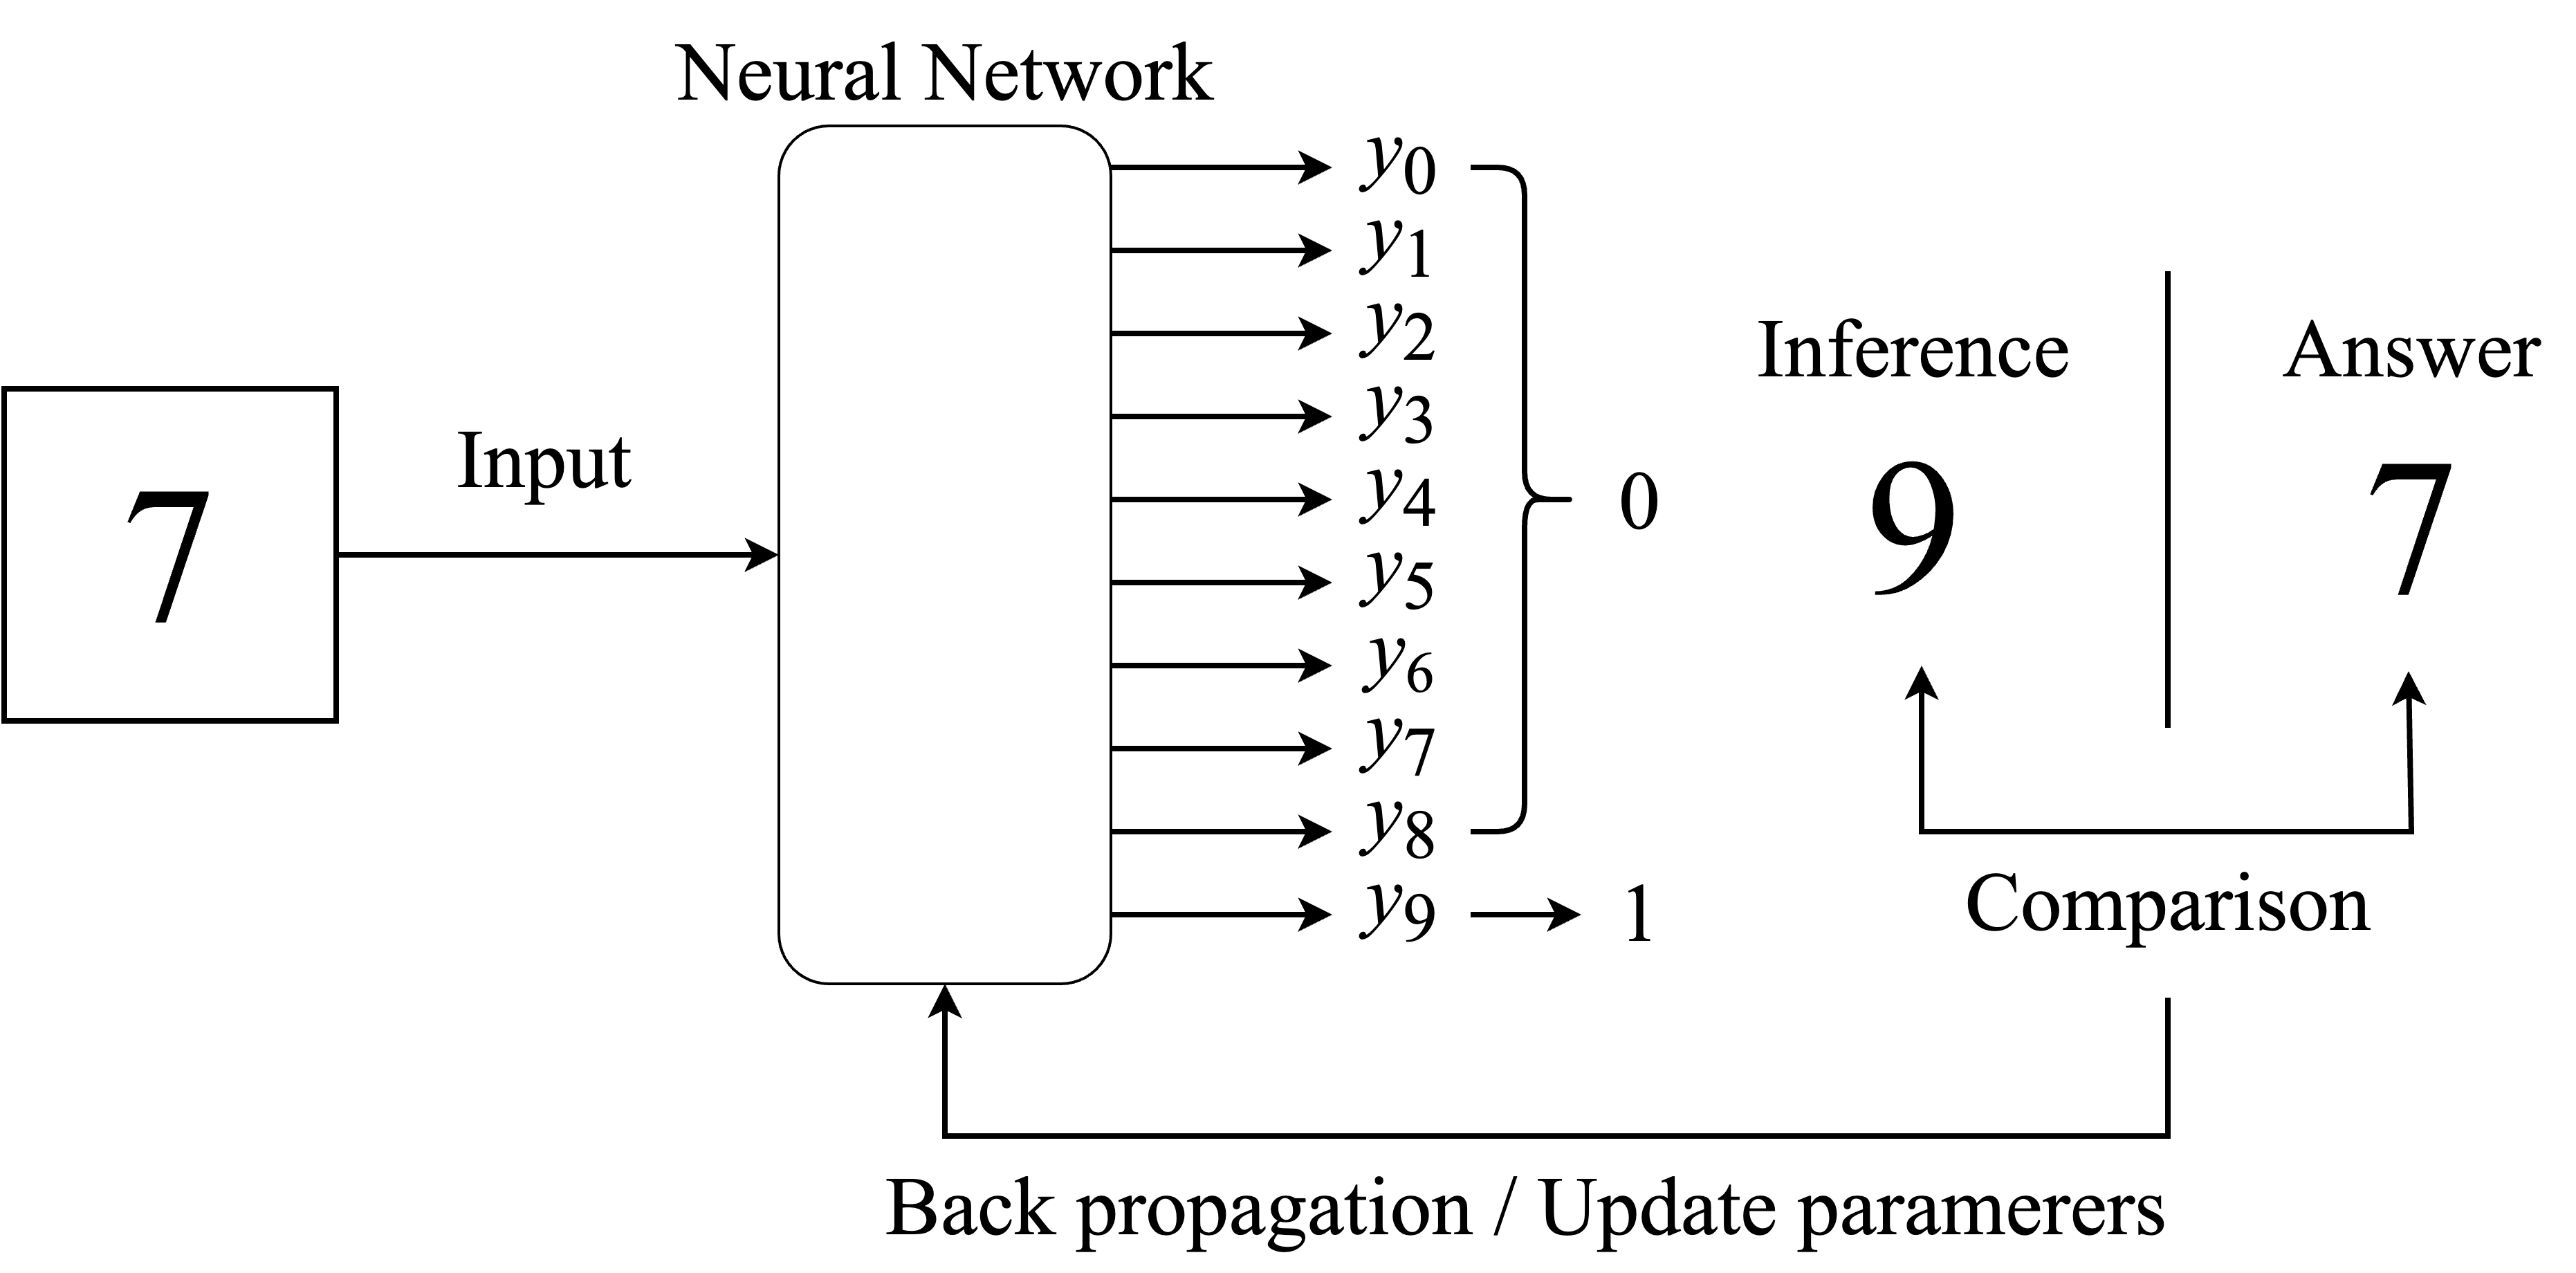
\includegraphics[scale = 0.1]{./chapter2/NN_study.png}
    \caption{Neural Networkにおける学習の流れ}
    \label{fig_study}
  \end{center}
\end{figure}

このとき,実際の答えは7だが推論の結果は9となり不正解になる.そこで両者を比較し誤差逆伝搬を行うことでNeural Network内の重みをどのように変更すれば推論を正解に近づけることができるかを求める.そして重みを更新していき推論が正解に近づいていくように変更していくのがNeural Networkにおける機械学習である

% ******************************************************
% CNN
% ******************************************************
\section{CNN}
\subsection{学習の概要}
CNNとは畳み込みと呼ばれる画像処理を組み込んだNeural Networkの1種で,画像分類など画像を用いた学習を得意としている.Neural Networkに畳み込み層を追加したものがCNNであるが,畳み込み層における画像,フィルタがNeural Networkにおける入力,重みとなっている.複数の画像と複数のフィルタが存在し,計算は一般的なNeural Networkに比べ複雑になるが,構造の概念は図\ref{fig_NN}に示すものと変わらない.
CNNでは主に畳み込みとプーリングという処理を用いて画像の特徴を抽出し学習を行っている.


\subsection{畳み込みの計算}
畳み込み層を考える上で,図\ref{fig_conv}のように$I \times J$ピクセルの画像と$2 \times 2$の要素を持つフィルタが存在すると考える.
\begin{figure}[]
  \begin{center}
    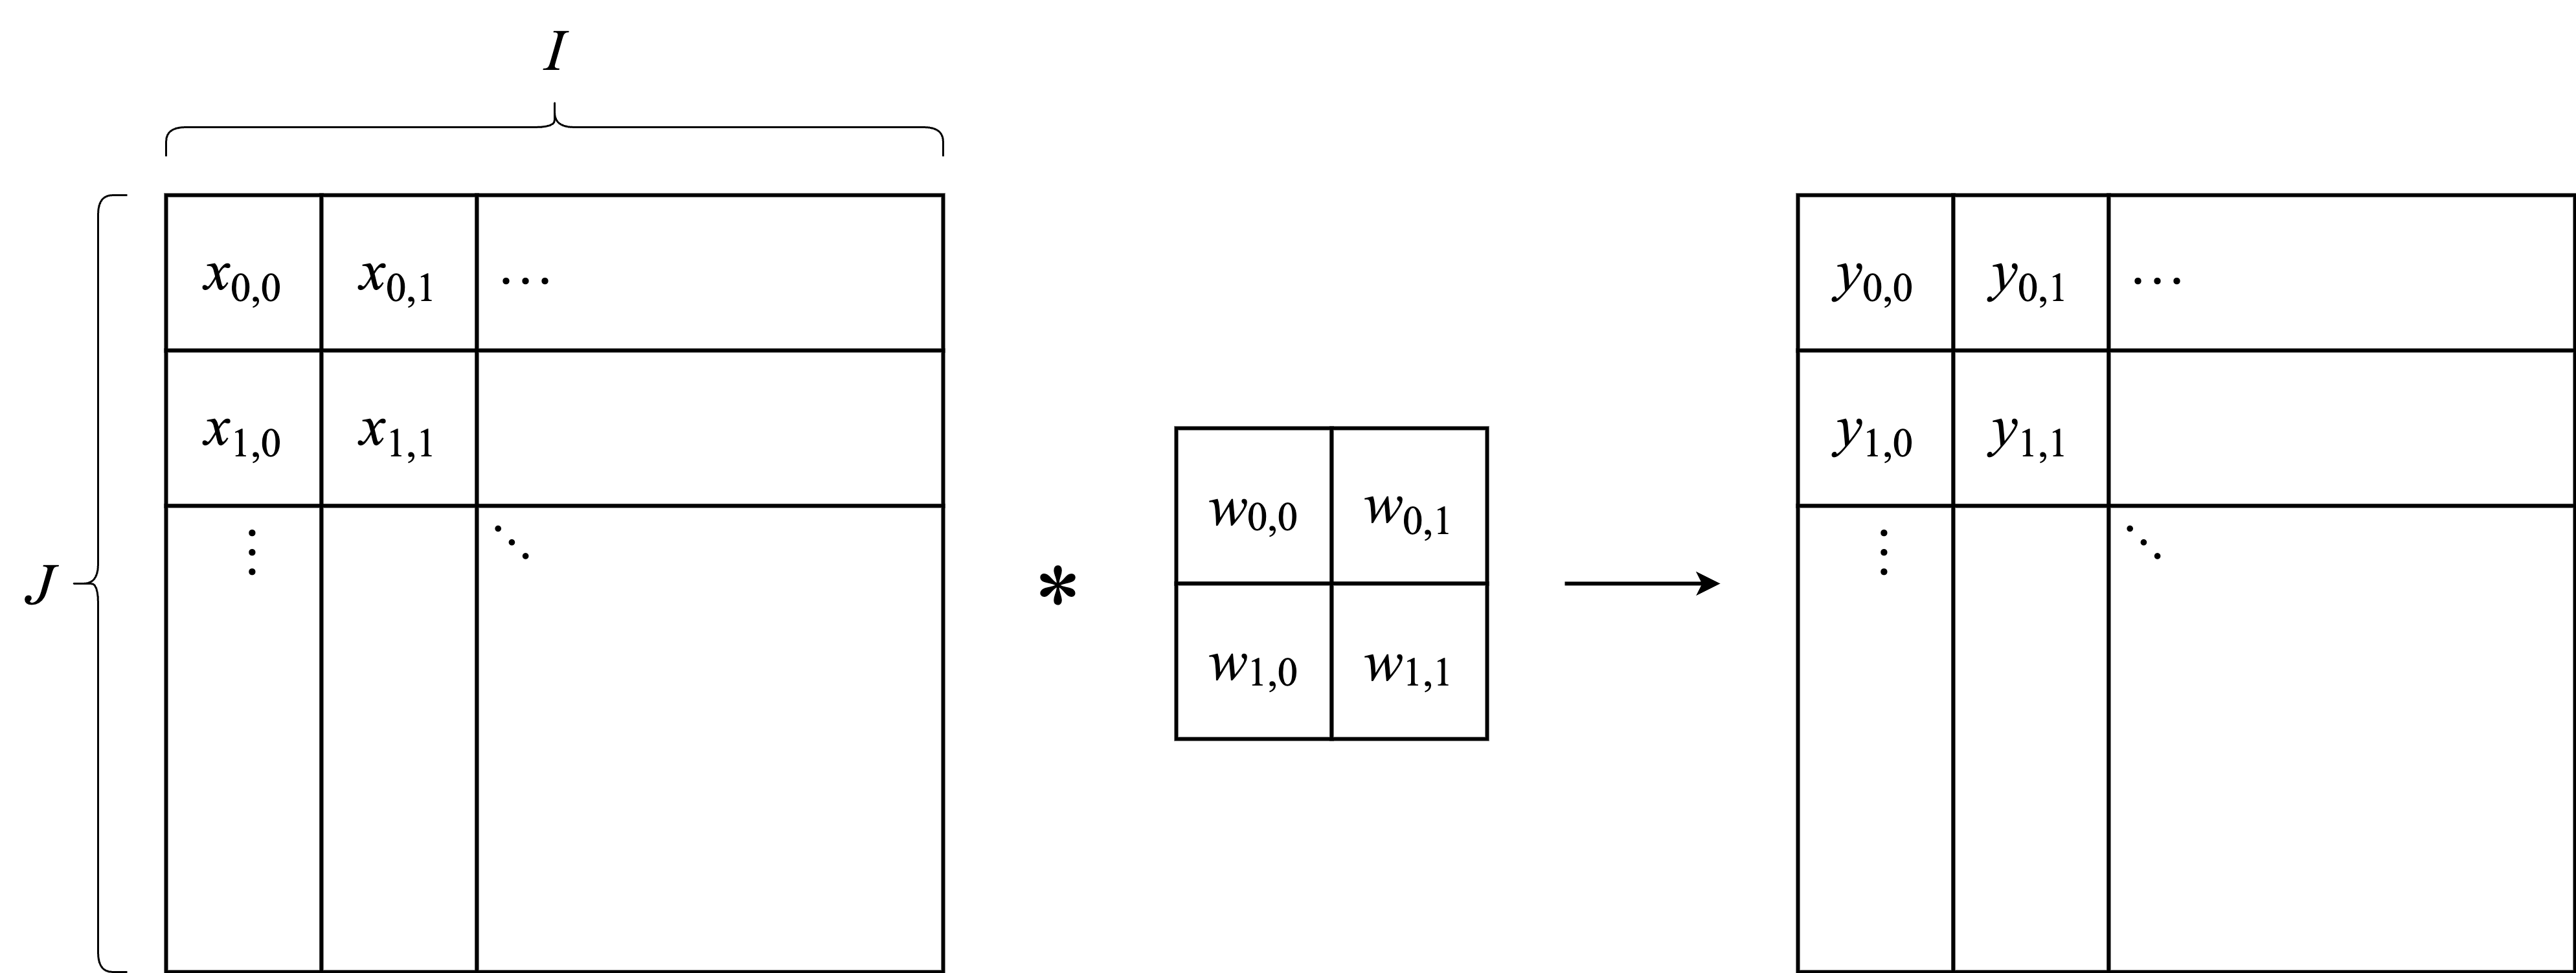
\includegraphics[scale = 0.08]{./chapter2/cnn_tatamikomi.png}
    \caption{畳み込み層での計算}
    \label{fig_conv}
  \end{center}
\end{figure}
ここでフィルタを$x_{11}$に重ねるように置き,各要素について乗算したものの和を出力とすると以下のように計算できる.
\begin{align*}
  y_{00} = x_{00}w_{00} + x_{01}w_{01} + x_{10}w_{10} + x_{11}w_{11}
\end{align*}

畳み込み層ではフィルターを1ピクセルずつスライドさせながら同じ計算をする.出力$y$のインデックスを$i,j$とし,フィルタのサイズを$W\times H$,とすると出力は以下の式で一般化できる.
\begin{align*}
  y_{ij} = \sum^{W-1}_{p=0} \sum^{H-1}_{q=0} x_{i-p,j-q}w_{pq}
\end{align*}
CNNではこの計算を繰り返していくことで画像の特徴を抽出する.

このままでは入力の画像に対し出力画像が1ピクセル分小さくなってしまうため,前後で画像サイズを変更したくない場合はパディングと呼ばれる入力画像の外側に情報を追加する処理を行う.よく使用されているのは0パディングと呼ばれる画像の外側1ピクセル分を0で埋め尽くす処理である.

またカラー画像を初期入力にした場合,チャンネル数はRGBの3chを持っている.フィルターは層ごとに増やしていき,フィルターの数だけ画像のch数は増えていく.これを図に表すと図\ref{fig_cnn_ch}のようになる.
\begin{figure}[]
  \begin{center}
    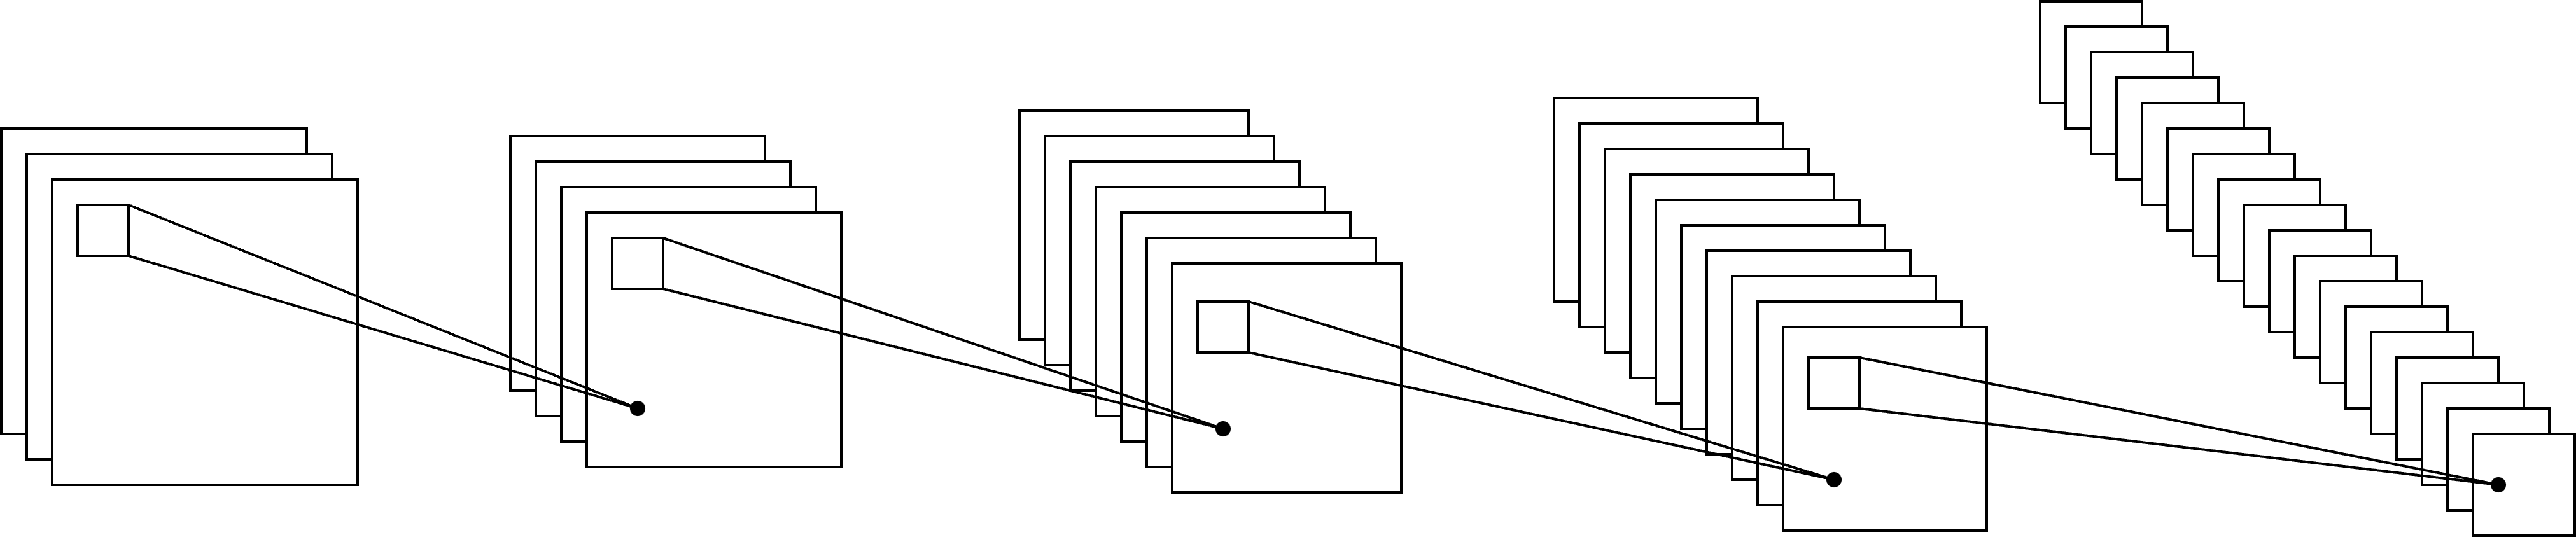
\includegraphics[scale = 0.08]{./chapter2/cnn_ch.png}
    \caption{畳み込み層でのchの増加}
    \label{fig_cnn_ch}
  \end{center}
\end{figure}

\subsection{プーリング層での計算}

\section{BinaryConnect}

